\documentclass{article}

% Recommended, but optional, packages for figures and better typesetting:
\usepackage{microtype}
\usepackage{graphicx}
\usepackage{subfigure}
\usepackage{booktabs} % for professional tables

% hyperref makes hyperlinks in the resulting PDF.
% If your build breaks (sometimes temporarily if a hyperlink spans a page)
% please comment out the following usepackage line and replace
% \usepackage{icml2021} with \usepackage[nohyperref]{icml2021} above.
\usepackage{hyperref}

\usepackage{url}            % simple URL typesetting
\usepackage{booktabs}       % professional-quality tables
\usepackage{amsfonts}       % blackboard math symbols
\usepackage{nicefrac}       % compact symbols for 1/2, etc.
\usepackage{microtype}      % microtypography


\usepackage{amsmath}
\usepackage{bm}
\usepackage{bbm}
\usepackage{xcolor}
\usepackage{graphicx}
\usepackage{overpic}
\usepackage{wrapfig}

\usepackage{siunitx}
\sisetup{output-exponent-marker=\ensuremath{\mathrm{e}}}

% \DeclareMathOperator*{\cgrad}{grad}
\newcommand{\cgrad}{\operatorname{grad}}
\DeclareMathOperator*{\cdiv}{div}
\DeclareMathOperator*{\dd}{d}
\DeclareMathOperator*{\diag}{diag}
\DeclareMathOperator*{\vect}{vec}
\DeclareMathOperator*{\real}{Re}

\newcommand{\code}[1]{\texttt{#1}}
\newtheorem{prop}{Proposition}
\newtheorem{thm}{Theorem}
\newtheorem{lem}{Lemma}

\newcommand{\michael}[1]{{\color{red}\sf{[Michael: #1]}}}
\newcommand{\charles}[1]{{\color{blue}\sf{[Charles: #1]}}}

\newcommand{\fakesection}[1]{%
  \par\refstepcounter{section}% Increase section counter
  \sectionmark{#1}% Add section mark (header)
  \addcontentsline{toc}{section}{\protect\numberline{\thesection}#1}% Add section to ToC
  % Add more content here, if needed.
}

% Attempt to make hyperref and algorithmic work together better:
\newcommand{\theHalgorithm}{\arabic{algorithm}}

% Use the following line for the initial blind version submitted for review:
\usepackage{icml2021}

% If accepted, instead use the following line for the camera-ready submission:
% \usepackage[accepted]{icml2021}

% The \icmltitle you define below is probably too long as a header.
% Therefore, a short form for the running title is supplied here:
\icmltitlerunning{Using Heavy-Tailed Self-Regularization Theory}

\begin{document}

\twocolumn[
\icmltitle{Using Heavy-Tailed Self-Regularization Theory to Characterize Correlations in and Perform Diagnostics on State-of-the-art Overparameterized Models} 

% It is OKAY to include author information, even for blind
% submissions: the style file will automatically remove it for you
% unless you've provided the [accepted] option to the icml2021
% package.

% List of affiliations: The first argument should be a (short)
% identifier you will use later to specify author affiliations
% Academic affiliations should list Department, University, City, Region, Country
% Industry affiliations should list Company, City, Region, Country

% You can specify symbols, otherwise they are numbered in order.
% Ideally, you should not use this facility. Affiliations will be numbered
% in order of appearance and this is the preferred way.
\icmlsetsymbol{equal}{*}

\begin{icmlauthorlist}
\icmlauthor{Charles H. Martin}{CC}
\icmlauthor{Michael W. Mahoney}{UCB}

\end{icmlauthorlist}

\icmlaffiliation{CC}{Department of Computer Science at Ben-Gurion University of the Negev, Israel.}
\icmlaffiliation{UCB}{ICSI and Department of Statistics at UC Berkeley, CA, USA.}

\icmlcorrespondingauthor{Omri Azencot}{azencot@cs.bgu.ac.il}

% You may provide any keywords that you
% find helpful for describing your paper; these are used to populate
% the "keywords" metadata in the PDF but will not be shown in the document
\icmlkeywords{Differential Geometry, Sequence Models}

\vskip 0.3in
]

% this must go after the closing bracket ] following \twocolumn[ ...

% This command actually creates the footnote in the first column
% listing the affiliations and the copyright notice.
% The command takes one argument, which is text to display at the start of the footnote.
% The \icmlEqualContribution command is standard text for equal contribution.
% Remove it (just {}) if you do not need this facility.

\printAffiliationsAndNotice{}  % leave blank if no need to mention equal contribution
% \printAffiliationsAndNotice{\icmlEqualContribution} % otherwise use the standard text.

%\begin{abstract}
%\end{abstract}


\section*{Introduction}

Understanding state-of-the-art overparameterized deep neural networks (DNNs) requires detailed empirical studies as well as the development of predictive theory in light of those studies. 
We use the theory of Heavy-Tailed Self-Regularization (HT-SR) to predict the generalization accuracy and improve the fine-tuning of (overparameterized) pretrained DNN models by capturing the dominant correlation structure.
HT-SR is based on Heavy-Tailed Random Matrix Theory (HT-RMT) and strongly-correlated systems theory from theoretical chemistry and theoretical physics, and methods based on it are implemented in the publicly-available \texttt{WeightWatcher} tool.
Using \texttt{WeightWatcher}, we can characterize HT structure in the empirical spectral densities (ESDs) of the layer weight matrices, and we can use this to predict trends in the reported test accuracies across hundreds of pretrained DNNs---without needing access to training or test data.
Going beyond popular norm-based metrics, we show that different metrics, which either depend on the scale or shap of the ESDs, exhibit a Simpson's paradox when varying DNN model depth versus regularization hyperparameters.
The familiar scale-based spectral norm metric behaves opposite to theoretical predictions, while the HT $\alpha$-metric acts as predicted.
The paradoxical behavior  can be resolved by combining these shape and scale metrics with the HT $\hat{\alpha}$ metric.
Finally, and with access to training data, we show how to
smooth out and capture the low rank structure to both accurately
predict the generalization errors and potentially improve
fine-tuning of pretrained DNNs.


%\michael{Here is Charles initial core dump of intro; still to refine and incorporate with rest of text.}
%We present our Theory of Heavy Tailed Self Regularization (HTSR) and
%its application to the (overparameterized)  Deep Neural Networks (DNNs) 
%to  predict the generalization accuracy and improve fine-tuning
%of pretrained models by capturing the dominant correlation structure.
%We analyze the correlations using techniques from 
%Heavy Tailed Random Matrix Theory (HT-RMT)
%and from  strongly correlated systems from theoretical
%chemistry and  physics.  
%We show how to predict trends in the reported test accuracies
%across hundreds of pretrained DNNs without needing access
%to training or test data by charactering the heavy tailed
%structure of the empirical spectral densities (ESD) of 
%the layer weight matrices.
%In doing so, we show that different metrics, which
%either depend on the shape or scale of the ESDs,
%exhbit a Simpson's paradox when varying DNN model depth
%vs regularization hyperparameters.
%In particular,  the familar scale-based spectral norm
%metric behaves opposite to theoretical predictions,
%whereas our HT alpha-metric acts as predicted.
%Moreover, the paradoxical behavior  can be resolved
%by combining these shape and scale metrics with
%our HT alpha-hat metric.
%Finally,  And with access to training data, we show how to
%smooth and capture the low rank structure to both accurately
%predict the generalization errors and potentially improve
%finetuning of pretrained DNNs.


\section*{Statistical Mechanics and Heavy-Tailed Self-Regularization}

%\citep{MM17_TR} is Charles: Rethinking generalization requires revisiting old ideas: statistical mechanics approaches and complex learning behavior''
%
%\citep{MM18_TR} is Charles: ``Implicit Self-Regularization in Deep Neural Networks: Evidence from Random Matrix Theory and Implications for Learning''
%
%\citep{MM19_HTSR_ICML} is Charles: ``Traditional and Heavy-Tailed Self Regularization in Neural Network Models''
%
%\citep{MM20_SDM} is Charles: ``Heavy-Tailed {U}niversality Predicts Trends in Test Accuracies for Very Large Pre-Trained Deep Neural Networks''
%
%\citep{MM19_KDD} is Charles: ``Statistical Mechanics Methods for Discovering Knowledge from Modern Production Quality Neural Networks''

Recently, RMT was applied to analyze empirically the weight matrices of DNNs, including both production quality, pretrained models such as AlexNet and Inception, and smaller models trained from scratch, such as LeNet5 and a miniature-AlexNet~\citep{MM18_TR} (see also \citep{MM17_TR, MM18_TR, MM19_HTSR_ICML, MM20_SDM, MM19_KDD}).
Building on these empirical results, 
\citet{MM18_TR} developed a phenomenological theory, based in statistical mechanics (as opposed to statistical learning theory), to identify ``5+1 Phases of Training,'' 
corresponding to increasing amounts of implicit self-regularization.
These phases can be observed during the training process as well as in the final learned (pretrained) DNNs.
For smaller and/or older DNNs, this implicit self-regularization is like traditional Tikhonov regularization, in that there is a ``size scale'' separating signal from noise.
For state-of-the-art (SOTA) DNNs, however, they identified a novel form of \emph{Heavy-Tailed Self-Regularization} (HT-SR).
This is similar to the self-organization seen in the statistical physics of disordered systems, such classical models of actual spiking neural activity; and 
it results from correlations arising at all size scales.
For DNNs, this arises due to the training process itself, when applied to very overparameterized models.

In the HT-SR theory, one analyzes the eigenvalue spectrum, or empirical spectral density (ESD) 
of the associated layer correlation matrices~\citep{MM18_TR,MM19_HTSR_ICML,MM20_SDM}.
and uses this to characterizes the amount and form of correlation present in the DNN's weight matrices.
For each layer weight matrix $\mathbf{W}$, if we compute the eigenvalue spectrum of 
$ \mathbf{X} = \frac{1}{N}\mathbf{W}^{T}\mathbf{W} $
then HT-SR theory characterizes the correlations in a weight matrix by fitting its ESD, $\rho(\lambda)$.
to a truncated Power Law (TPL) distribution,  $\rho(\lambda)\sim\lambda^{-\alpha} $.
%
The original work on HT-SR showed that among numerous publicly-available SOTA models, for nearly every $\mathbf{W}$,  the tail of the ESDs can be fit to a  TPL, and that Power Law (PL) exponents $\alpha$ nearly all lie within the range $\alpha\in(1.5,5)$~\citep{MM18_TR,MM19_HTSR_ICML,MM20_SDM}.
%
%%As for the mechanism responsible for these properties, statistical physics offers several possibilities~\citep{SornetteBook,nishimori01}, e.g., self organized criticality~\citep{SOC87,SOCat25yrs} or multiplicative noise in the stochastic optimization algorithms used to train these models~\citep{HodMah20A_TR,SorCon97}.
%%Alternatively, related techniques have been used to analyze correlations and information propogation in actual spiking neurons~\citep{SYYRP11,YKYP14}.
%%Our meta-analysis does not require knowledge of mechanisms; and it is not even clear that one mechanism is responsible for every case.
%
Crucially, HT-SR theory predicts that smaller values of $\alpha$ should correspond to models with better correlation over multiple size scales and thus to better models,
and therefore higher generalization accuracies.
%%The notion of ``size scale'' is well-defined in physical systems, to which this style of analysis is usually applied, but it is less well-defined in CV and NLP applications.
%%Informally, it would correspond to pixel groups that are at a greater distance in some metric, or between sentence parts that are at a greater distance in text.
%%Relatedly, previous work observed that smaller exponents $\alpha$ correspond to more implicit self-regularization and better generalization, and that we expect a linear correlation between $\hat{\alpha}$ and model quality~\citep{MM18_TR,MM19_HTSR_ICML,MM20_SDM}.


\section*{Overall approach}

Test accuracies have been reported online for publicly-available pretrained pyTorch models~\citep{osmr}.
These models have been trained and evaluated on labeled data, using standard techniques.  
We do not have access to this data, and we have not trained any of the models ourselves. 
Our methodological approach is thus similar to a statistical meta-analysis, common in biomedical research, but uncommon in machine learning.
%
To evaluate the quality of SOTA DNNs, we consider the following metrics:
Frobenius Norm, $\Vert\mathbf{W}\Vert^{2}_{F}=\Vert\mathbf{X}\Vert_{F}=\sum\nolimits_{i=1}^{M} \lambda_{i}$; 
Spectral Norm, $\Vert\mathbf{W}\Vert_{\infty}^{2}=\Vert\mathbf{X}\Vert_{\infty}=\lambda_{max}$;
Weighted Alpha, $\hat{\alpha}=\alpha\log\lambda_{max}$; and
$\alpha$-Shatten Norm, $\Vert\mathbf{W}\Vert^{2\alpha}_{2\alpha}=\Vert\mathbf{X}\Vert^{\alpha}_{\alpha}=\sum\nolimits_{i=1}^{M}\lambda_{i}^{\alpha}$. 
%\begin{eqnarray*}
%& & \text{Frobenius Norm: $\Vert\mathbf{W}\Vert^{2}_{F}=\Vert\mathbf{X}\Vert_{F}=\sum\nolimits_{i=1}^{M} \lambda_{i}$ } \\
%& & \text{Spectral Norm: $\Vert\mathbf{W}\Vert_{\infty}^{2}=\Vert\mathbf{X}\Vert_{\infty}=\lambda_{max}$ } \\
%& & \text{Weighted Alpha: $\hat{\alpha}=\alpha\log\lambda_{max}$ } \\
%& & \text{$\alpha$-Shatten Norm: $\Vert\mathbf{W}\Vert^{2\alpha}_{2\alpha}=\Vert\mathbf{X}\Vert^{\alpha}_{\alpha}=\sum\nolimits_{i=1}^{M}\lambda_{i}^{\alpha}$. }
%\end{eqnarray*}
To perform diagnostics on potentially-problematic DNNs, we will decompose $\hat{\alpha}$ into its two components, $\alpha$ and $\lambda_{max}$.
One determines $\alpha$ for a given layer by fitting the ESD of that layer's weight matrix to a truncated PL, using the commonly accepted Maximum Likelihood method~\citep{CSN09_powerlaw,ABP14}.
Computations were performed with the publicly-available \texttt{WeightWatcher} tool (version 0.2.7)~\citep{weightwatcher_package}.


\section*{Predicting Trends in the Quality of State-of-the-art Models}


%XXX.  ABSTRACT FROM \citep{MM20a_trends_TR}: ``Predicting trends in the quality of state-of-the-art neural networks without access to training or testing data''

In many applications, one works with DNN models trained by someone else.
For such pretrained models, one may not have access to training data or test data.
Moreover, one may not know details about the model, e.g., the specifics of the training data, the loss function, the hyperparameter values, etc.
(So, one is \emph{not} training models, one is validating pretrained models.)
Given one or many pretrained models, it is a challenge to say anything about the expected performance or quality of the models.
We have applied HT-SR theory to provide a detailed meta-analysis of hundreds of publicly-available pretrained models, examining both norm based capacity control metrics (from statistical learning theory) as well as PL based metrics (from HT-SR theory).

We consider a large suite of hundreds of publicly-available models, mostly from computer vision (CV) and natural language processing (NLP).
By now, there are many such state-of-the-art models that are publicly-available, e.g., 
hundreds of pretrained models in CV ($\ge 500$) and NLP ($\approx 100$).
For all these models, we have no access to training data or testing data, and we have no specific knowledge of the training/testing protocols. 
Thus, performing weight matrix analysis is a natural option.


We find that norm based metrics correlate well with reported test accuracies for well-trained models, but that they often cannot distinguish well-trained versus poorly-trained models.
We also find that PL based metrics can do much better---quantitatively better at discriminating among series of well-trained models with a given architecture; and qualitatively better at discriminating well-trained versus poorly-trained models.
These methods can be used to identify when a pretrained DNN has problems that cannot be detected simply by examining training/test accuracies.
%
%Here is a summary of our main results.
%First, norm-based metrics do a reasonably good job at predicting quality trends in well-trained CV/NLP models.
%Second, norm-based metrics may give spurious results when applied to poorly-trained models (e.g., models trained without enough data, etc.).
%For example, they may exhibit what we call Scale Collapse for these models. 
%Third, PL-based metrics can do much better at predicting quality trends in pretrained CV/NLP models.  
%In particular, 
%a weighted PL exponent (weighted by the log of the spectral norm of the corresponding layer) is 
%quantitatively better at discriminating among a series of well-trained versus very-well-trained models
%within a given architecture series; and
%the (unweighted) average PL exponent is 
%qualitatively better at discriminating well-trained versus poorly-trained models.
%Fourth, PL-based metrics can also be used to characterize fine-scale model properties, including what we call layer-wise Correlation Flow, in well-trained and poorly-trained models; and they can be used to evaluate model enhancements (e.g., distillation, fine-tuning, etc.).
See Table~\ref{table:results} for an overview summary of our results.

Our work provides a theoretically-principled empirical evaluation---by far the largest, most detailed, and most comprehensive to date---and it uses HT-SR theory.
%
%\citep{BFT17_TR} is Bartlett: ``Spectrally-normalized margin bounds for neural networks''
%\citep{LMBx18_TR} is Poggio: ``A surprising linear relationship predicts test performance in deep networks''
There is related work \citep{BFT17_TR,LMBx18_TR}, but that work provides generalization bounds, modifies the models, requires access to data, etc., and so is quite different.



\begin{table}[t]
\small
\begin{center}
\begin{tabular}{|p{0.83in}|c|c|c|c|}
\hline
  & $\log\Vert\cdot\Vert^{2}_{F}$ & $\log\Vert\cdot\Vert^{2}_{\infty}$ & $\hat{\alpha}$ & $\log\Vert\cdot\Vert^{\alpha}_{\alpha}$ \\
\hline

RMSE (mean) & 4.84 & 5.57 & 4.58& 4.55 \\
RMSE (std) & 9.14 & 9.16 & 9.16& 9.17 \\
\hline
R2 (mean) & 3.9 & 3.85 & 3.89& 3.89 \\
R2 (std) & 9.34 & 9.36 & 9.34& 9.34 \\
\hline
Kendal-$\tau$ (mean) & 3.84 & 3.77 & 3.86& 3.85 \\
Kendal-$\tau$ (std) & 9.37 & 9.4 & 9.36& 9.36 \\
\hline

\hline
\end{tabular}
\end{center}
\caption{Comparison of linear regressions for different average Log Norm and Weighted Alpha metrics across 5 CV datasets, 17 architectures, covering \
108 (out of $>400$) different pretrained~DNNs.
}
\label{table:results}
\end{table}


\section*{A Simpson's Paradox---and the Need for Finer-scale Analysis}

%\citep{JNBx19_fantastic_TR} is the terrible fantastic paper: ``Fantastic Generalization Measures and Where to Find Them''
%
%\citep{JFYx20_contest_v10} is the contest: ``{NeurIPS} 2020 Competition: Predicting Generalization in Deep Learning (Version 1.0)''
%
%\citep{BHO75} is Bickel: ``Sex Bias in Graduate Admissions: Data from Berkeley''

\begin{figure}[t!] 
    \centering
    \subfigure[Log Spectral Norm]{
       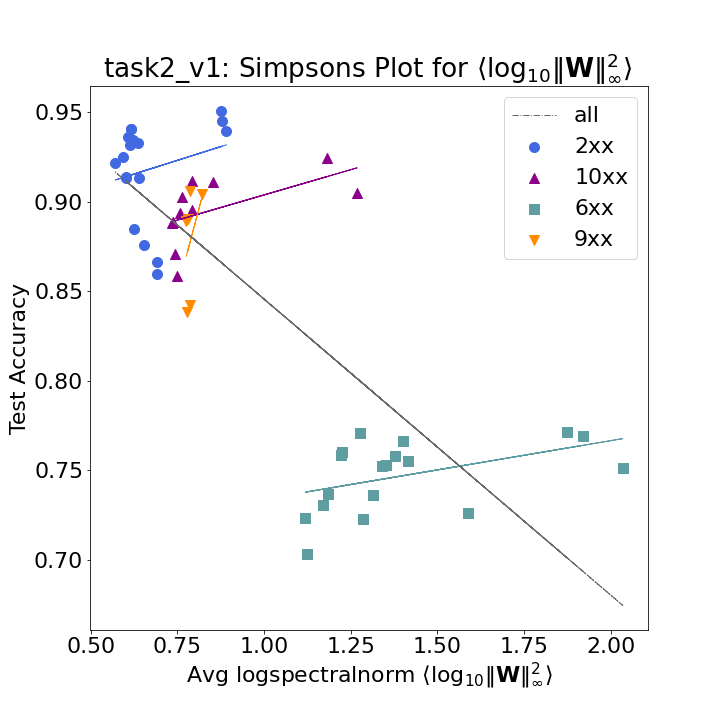
\includegraphics[width=3.5cm]{img/simpsons-task2-logspectralnorm.png}
    }
    \subfigure[Weighted Alpha $\hat{\alpha}$]{
       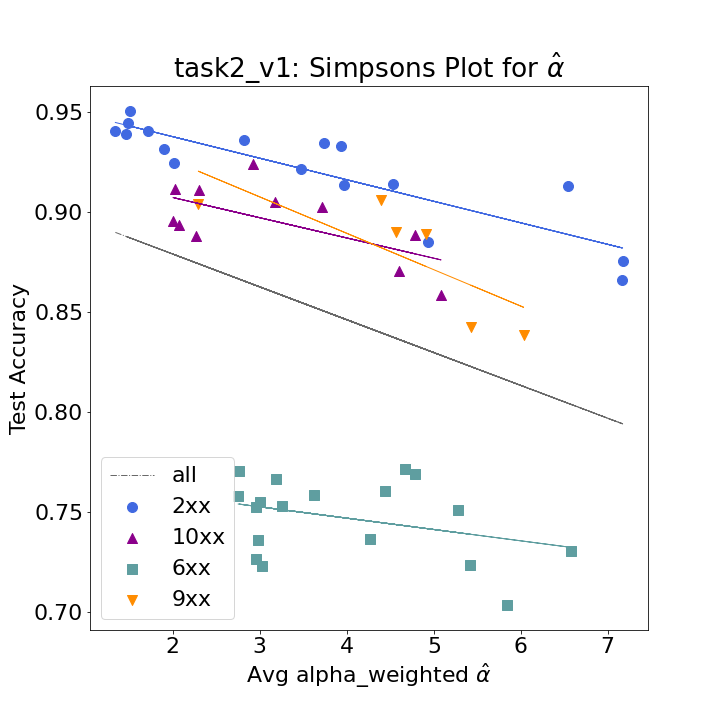
\includegraphics[width=3.5cm]{img/simpsons-task2-alpha_weighted.png}
    }
    \caption{Test accuracy as a function of 
             the Log Spectral Norm and 
             the (HT-SR) Weighted Alpha ($\hat{\alpha}$) metrics,
             as model hyperparameters and depth are varied. 
             Models are from the NeurIPS 2020 ``Predicting Generalization'' contest.
             A Simpson's paradox is clearly visible.
            }
    \label{fig:simpsons}
\end{figure} 

Subsequent to the development of HT-SR theory, and our initial results on analyzing pretrained models at scale, there was at NeurIPS 2020 a ``Predicting Generalization'' workshop and contest \citep{JNBx19_fantastic_TR, JFYx20_contest_v10}.
This contest made publicly-available pretrained models.
This corpus of models was much more narrow (in terms of domain) but more extensive (in terms of depth and hyperparameter variation) than the previous SOTA corpus we considered~\citep{osmr}.

In particular, we apply HT-SR theory to predict the generalization accuracies of the pretrained models provided in this contest, as a function of both model depth ($L$) and the solver hyperparameters (batch size, dropout, weight decay), and we compare quality metrics that describe the norm-based scale and the HT/PL shape of the model layer weight matrices.  
See Figure~\ref{fig:simpsons} for a summary.
For norm-based metrics, we identify what amounts to a Simpson’s paradox \citep{BHO75}, in which scale and shape metrics show opposite behavior, depending on whether the data are partitioned by depth or solver hyperparameters values.
Since $\hat{\alpha}$ combines both scale and shape information, it resolves the paradox.

%\charles{We apply our theory of Heavy Tailed Self-Regularization (HTSR) to predict the generalization accuracies of the pretrained models provided in this contest, as a function of both model depth (L) and the solver hyperparameters (batch size, dropout, weight decay), and compare quality metrics that describe both the heavy-tailed shape and norm-based scale of the model layer weight matrices.  In doing so, we identify what amounts to a Simpson’s paradox, in which shape and scale metrics show opposite behavior, and a combine metric resolves the paradox}


\section*{Conclusion}

The HT-SR theory underlying our analysis is quite different than theoretical approaches popular in machine learning, and it is quite different than typical statistical mechanics approaches to DNNs \citep{BKPx20}.
%
%Recently, however, work motivated by HT-SR theory has 
%demonstrated that multiplicative noise in stochastic optimization leads to heavy tails~\citep{HodMah20A_TR,GSZ20_TR}; 
%provided a random matrix analysis of random {F}ourier features, going beyond the {G}aussian kernel, to provide a precise phase transition and illustrate the corresponding double descent~\citep{ZCM20_TR}; 
%provided exact expressions for double descent and implicit regularization via a notion of surrogate random design \citep{DLM19_Exact_TR}; 
%demonstrated that good classifiers are abundant in the interpolating regime \citep{TKM20_TR};
%shown how injecting noise into hidden states of recurrent NNs leads to implicit regularization~\citep{LEHM21_TR,Mah12}; and 
%shown that analogous phase transitions hold for the {C}olumn {S}ubset {S}election and the {N}ystrom method~\citep{DKM20_TR}. 
%We expect that the empirical results identified by tools from HT-SR theory will provide guidance and constraints for future development of overparameterized machine learning models.
%
However, recent work, work motivated by HT-SR theory, has begun to appear
\citep{HodMah20A_TR,GSZ20_TR, ZCM20_TR, DLM19_Exact_TR, TKM20_TR, LEHM21_TR,Mah12, DKM20_TR}. 
We expect that the empirical results and theoretical insights HT-SR theory provides will provide guidance and constraints for future development of overparameterized machine learning models.



\bibliographystyle{icml2021}
\bibliography{dnns}


\end{document}


